\chapter{Optimisation}
\section{Motivation}
\begin{quote}
    \textit{"Users expect miracles! \dots Data management systems can actually accommodate some \dots - Holger Pirk"}
\end{quote}
\begin{itemize}
    \item Users want zero-overhead, the system should be as fast as hand-written \& optimised code.
    \item The database is expected to learn from data (e.g second run of a query is faster)
    \item System must be highly flexible (users can create relations, indices, build complex queries without needing to upgrade/reconfigure/recompile any part of the DBMS) 
\end{itemize}
In reality current \textit{DBMS} generally succeed in meeting these \textit{miraculous} expectations.

\subsection{Query Optimisers vs Optimising Compilers}
A query optimiser is similar to a compiler's optimiser:
\begin{itemize}
    \item Representation of code is transformed through several representations, some logical (e.g AST, three address code), some physical (e.g x86 specific IR, assembly representation)
    \item Correctness under optimisations (\textbf{primary objective}), performance of optimiser queries (\textbf{secondary objective}).
    \item Limitations on time to optimise (e.g developers don't want to wait excessively long to compile simple programs)
\end{itemize}
The main difference is timing of access to code and input data.
\begin{center}
    \begin{tabular}{l l l}
        & \textbf{Code/Query} & \textbf{Input Data} \\
        \textbf{Compiler Optimiser} & At compile time & Unknown \\
        \textbf{Query Optimiser} & At query time & Known before query \\
    \end{tabular}
\end{center}

\begin{sidenotebox}{Profile Guided Optimisation}
    A compiler optimiser (at compile) does not have access to the input data (at runtime). However this is not entirely \textit{technically} true. We can compile an instrumented version of the code, run with some representative input data, profile and provide this feedback to the compiler to guide optimisation.
    \begin{minted}{bash}
g++ -fprofile-generate myprog.cpp # Compile instrumented version
./myprog.cpp                      # Generates myprog.gcda
g++ -fprofile-use myprog.cpp      # Use profile when optimising
    \end{minted}
\end{sidenotebox} 

Correctness is difficult.
\begin{itemize}
    \item ANSI SQL semantics are not formally defined (though some have been \href{https://dl.acm.org/doi/10.1145/111197.111212}{developed}).
    \item Need to test against complex queries, numerous edge cases, with many combinations of optimisations (much the same as with compiler's optimisers).
\end{itemize}

\begin{sidenotebox}{Fuzzing}
    One common practice for testing compilers (and DBMS) is to randomly generate potential queries, and then test for differences in results from optimised and un-optimised.
    \begin{center}
        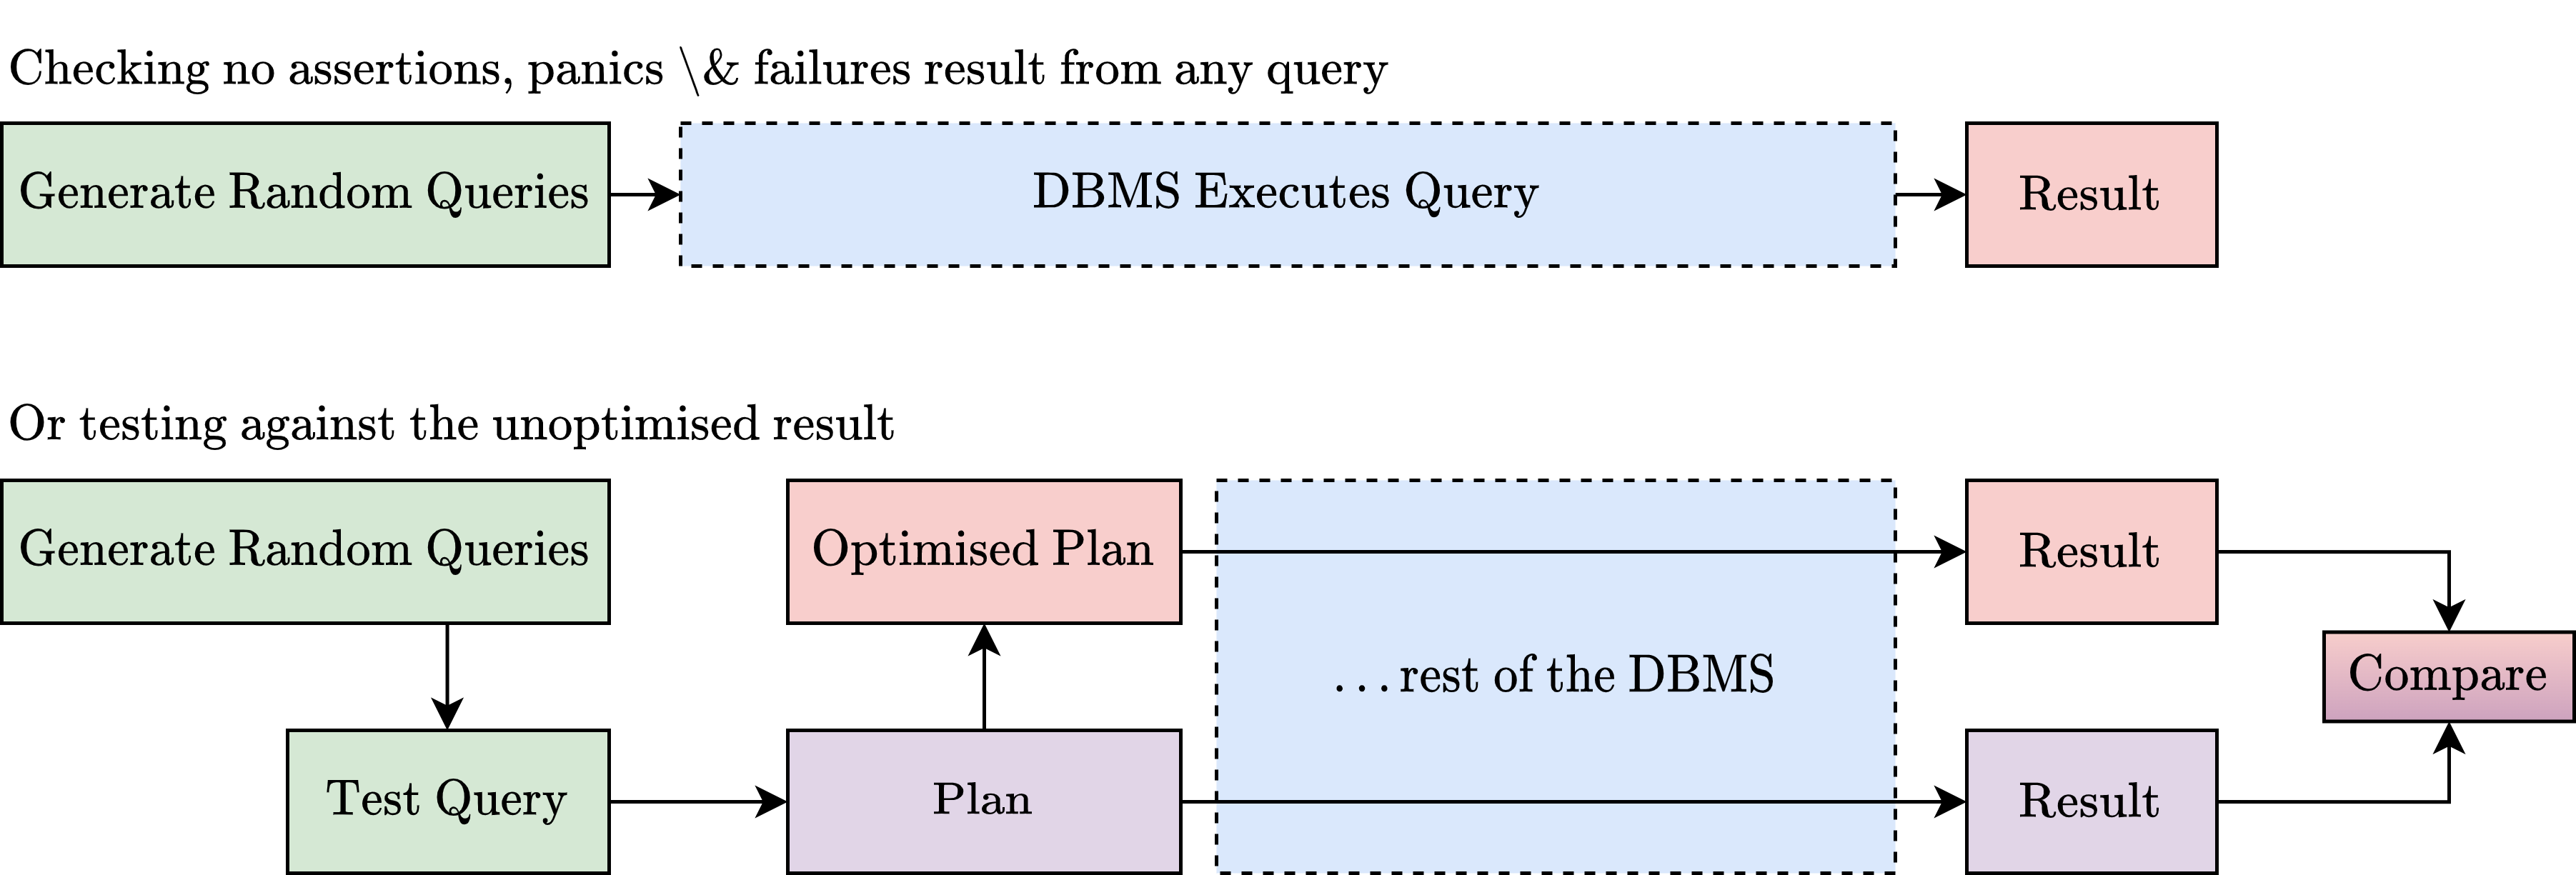
\includegraphics[width=.8\textwidth]{optimisation/images/fuzzing.drawio.png}
    \end{center}
    For example \href{https://github.com/anse1/sqlsmith}{sqlsmith} can be used to generate random SQL queries, and has been used to test and find bugs in Postgres, sqlite3, monetdb and more (see the \href{https://github.com/anse1/sqlsmith/wiki#score-list}{score list}).
\end{sidenotebox}

\subsection{Query Equivalence}
\begin{definitionbox}{Semantic Equivalence}
    Plans are \textit{semantically equivalent} if they provable produce the same output on any dataset.
\end{definitionbox}
\begin{definitionbox}{Closure (Mathematics)}
    (\textit{Simplified}) A set is closed under an operation if the operation produces elements of the same set.
    \begin{itemize}
        \item $\mathbb{N}$ is closed under $+$, but not under $-$ (can produce negative numbers)
        \item \textit{Relational algebra} is closed (the set of possible relations is closed under the operators of the algebra).
    \end{itemize}
\end{definitionbox}
\begin{center}
    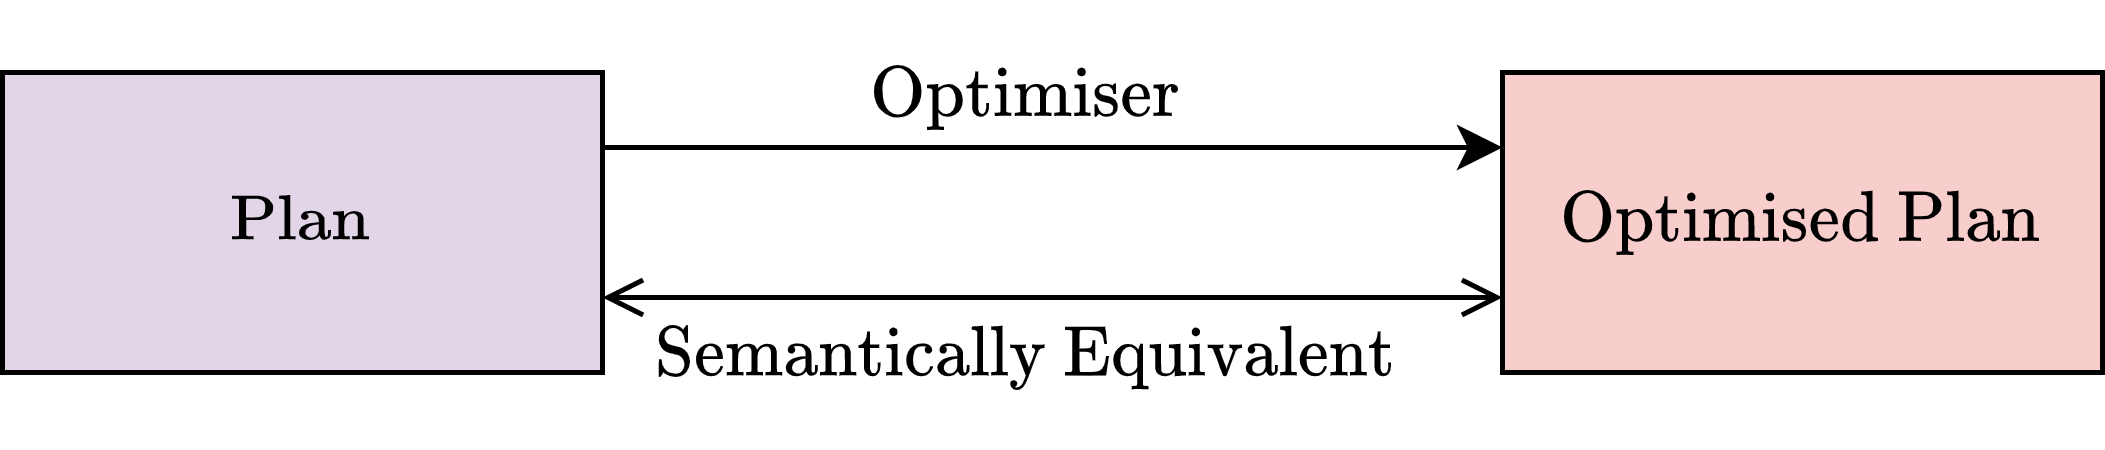
\includegraphics[width=.7\textwidth]{optimisation/images/semantic_equivalence.drawio.png}
\end{center}
As \textit{relational algebra} is closed, operators are easily composable.
\begin{itemize}
    \item We can determine equivalences between compositions of operators.
    \item Substitutions of a part of a plan with an equivalent, results in a new equivalent plan.
    \item We can use this to transform plans into more optimal (but equivalent) plans. 
\end{itemize}

\section{Peephole Transformations}
\begin{quote}
    \textit{"An equivalent transformation of a subplan is an equivalent transformation of the entire plan."}
\end{quote}
A set of rules for transforming small subplans (peephole) is applied while traversing the plan.

\begin{sidenotebox}{WACC Peephole}
    This is the same idea as peephole optimisations discussed in the WACC project and 50006 - Compilers.
    \begin{minipage}{.49\textwidth}
        \begin{minted}{asm}
mov r1, r1 ; redundant move
        
        \end{minted}
    \end{minipage} \hfill \begin{minipage}{.49\textwidth}
        \begin{minted}{asm}
str r4, [sp, #8] ; overwritten store 
str l3, [sp, #8]
        \end{minted}
    \end{minipage}
\end{sidenotebox}

\begin{itemize}
    \item Need some order with which to traverse the plan
    \item Need a set of patterns/rules for 
\end{itemize}

% plan cycles
% diverging plans

\section{Logical \& Physical Optimisation}

\subsection{Rule Based Logical Optimisation}

\subsubsection{Selection Pushdown}

\subsubsection{Selection Ordering}

\subsubsection{Implication}

\section{Cost Based Logical Optimisation}
% heuristics
% histograms
% multidimensional histograms


\section{Physical Optimisation}
% Cost metrics
% function calls, produced tuples, page faults, max(I/O, CPU), intermediate sizes

\subsection{Rule Based Physical Optimisation}

% data structure choice
% sort merge join when input data is sorted
% using existing indices

\subsection{Cost Based Physical Optimisation}
% parameters (buffer pool size, data, hardware - accelerators/extensions)


\section{SparkSQL}
% spark system architecture
% catalyst optimiser
\unfinished
